\documentclass[dvipdfmx]{jarticle}
\usepackage{tikz}
\usetikzlibrary{calc}
\pagestyle{empty}
%\include{cmacros}
\begin{document}
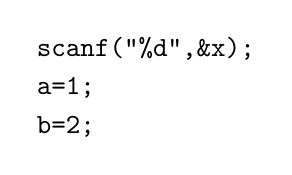
\begin{tikzpicture}
   \node[anchor=west] at ($0*(0,-0.5)$) {\texttt{scanf("\%d",\&x);}};
   \node[anchor=west] at ($1*(0,-0.5)$) {\texttt{a=1;}};
   \node[anchor=west] at ($2*(0,-0.5)$) {\texttt{b=2;}};
\end{tikzpicture}
%   \begin{pspicture}(0,0)(5,4)
%    \setlength{\normalgap}{0.4pt}
%    \setlength{\indentval}{0.2pt}
%    \setlength{\rowheight}{7.5pt}
%    \setlength{\colpos}{0pt}
%    \cstatline{scanf("\% d",\& x);}\nnextline
%    \cstatline{a=1;}\nnextline
%    \cstatline{b=2;}\nnextline
%    \cstatline{c=a+b;}\nnextline
%    \cstatline{if(x>0) a=3;}\nnextline
%    \cstatline{d=b;}\nnextline
%    \cstatline{c=a+b;}
%   \end{pspicture}
\end{document}

